\section{Question 1}
    State space representation from differential equations

    \subsection{a)} 
    $2\ddot{x} + 4\dot{x} + 4x=3u$, where the state vector is 
    $\begin{bmatrix}
        x \\
        \dot{x}
    \end{bmatrix}$.
    The out put is x.
    \subsubsection{solution}
    $\ddot{x} + 2\dot{x} + 2x=1.5u$ $\Rightarrow$ 
    $\left\{
        \begin{array}{lr}
        \dot{x} = 0x + \dot{x} \\
        \ddot{x} = -2x -2\dot{x} + 1.5u
        \end{array}
    \right.$, thus

    \begin{align}
        \dot{\textbf{x}} &=
        \begin{bmatrix}
            \dot{x} \\
            \ddot{x}
        \end{bmatrix} = 
        \begin{bmatrix}
            0 & 1 \\
            -2 & -2
        \end{bmatrix}
        \begin{bmatrix}
            x \\
            \dot{x}
        \end{bmatrix} + 
        \begin{bmatrix}
            0\\
            1.5
        \end{bmatrix}
        u
        \\
        \dot{\textbf{y}} &=
        \begin{bmatrix}
            x
        \end{bmatrix} =
        \begin{bmatrix}
            1 & 0
        \end{bmatrix}
        \begin{bmatrix}
            x \\
            \dot{x}
        \end{bmatrix} + 
        \begin{bmatrix}
            0
        \end{bmatrix}
        u
    \end{align}

    We get:

    \begin{equation}
        \textbf{A} =
        \begin{bmatrix}
            0 & 1 \\
            -2 & -2
        \end{bmatrix}, 
        \textbf{B} =
        \begin{bmatrix}
            0\\
            1.5
        \end{bmatrix}, 
        \textbf{C} =
        \begin{bmatrix}
            1 & 0
        \end{bmatrix}, 
        \textbf{D} =
        \begin{bmatrix}
            0
        \end{bmatrix}
    \end{equation}

    \subsection{b)} 
    $2\ddot{x} + 4\dot{x} + 4x=3u$, where the state vector is 
    $\begin{bmatrix}
        x + \dot{x} \\
        \dot{x}
    \end{bmatrix}$.
    The out put is x.

    \subsubsection{solution}
    $\left\{
        \begin{array}{lr}
        \dot{x} + \ddot{x} = \dot{x} + (-2x -2\dot{x} + 1.5u) = -2(x + \dot{x}) + \dot{x} + 1.5u\\
        \ddot{x} = -2x -2\dot{x} + 1.5u = -2(x + \dot{x}) + 0\dot{x} + 1.5u \\
        x = (x + \dot{x}) + (-1)\dot{x}
        \end{array}
    \right.$, thus

    \begin{align}
        \dot{\textbf{x}} &=
        \begin{bmatrix}
            \dot{x} + \ddot{x}\\
            \ddot{x}
        \end{bmatrix} = 
        \begin{bmatrix}
            -2 & 1 \\
            -2 & 0
        \end{bmatrix}
        \begin{bmatrix}
            x + \dot{x}\\
            \dot{x}
        \end{bmatrix} + 
        \begin{bmatrix}
            1.5\\
            1.5
        \end{bmatrix}
        u
        \\
        \dot{\textbf{y}} &=
        \begin{bmatrix}
            x
        \end{bmatrix} =
        \begin{bmatrix}
            1 & -1
        \end{bmatrix}
        \begin{bmatrix}
            x + \dot{x}\\
            \dot{x}
        \end{bmatrix} + 
        \begin{bmatrix}
            0
        \end{bmatrix}
        u
    \end{align}

    We get:

    \begin{equation}
        \textbf{A} =
        \begin{bmatrix}
            -2 & 1 \\
            -2 & 0
        \end{bmatrix}, 
        \textbf{B} =
        \begin{bmatrix}
            1.5\\
            1.5
        \end{bmatrix}, 
        \textbf{C} =
        \begin{bmatrix}
            1 & -1
        \end{bmatrix}, 
        \textbf{D} =
        \begin{bmatrix}
            0
        \end{bmatrix}
    \end{equation}
    

    \subsection{c)}
    Using the A,B,C,D matrices found in parts (a) and (b), use Matlab's step command to simulate the step responses to both systems. How do these step responses compare and does that comparison make sense? 
    \subsubsection{solution}
    Matlab code:
    \lstinputlisting{codes/Question1c.m}
    Result:
    \begin{figure}[htp]
        \centering
        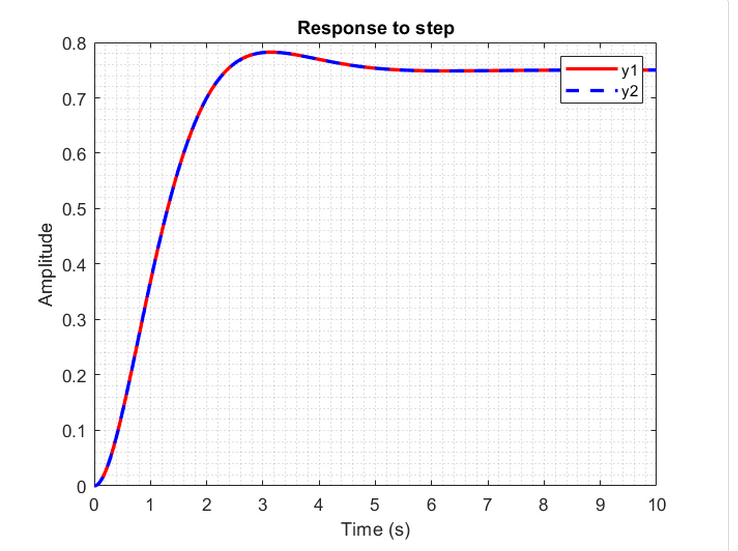
\includegraphics[width=15cm]{images/Q1_c_fig.png}
        \caption{Step Response}
        \label{fig:Q1c}
    \end{figure}

    We can tell from Fig.\ref{fig:Q1c} that the step responses are exactly the same.
    This make sense because we are representing the same system, and the output is the same for the two representations. 

\pagebreak